\chapter{Week 4: 9\textsuperscript{th} - 15\textsuperscript{th} February }

\begin{itemize*}
	\item Tune the Kalman Filter that uses a pure kinematic system model (i.e is independent of a control input matrix)
	\item Read up on non-linear control
	\item  Investigate the \gls{ekf} as it is commonly used in GPS systems 
\end{itemize*}

 \tocless\section{Tuning of a Kalman Filter that uses a pure kinematic}
This it was decided  to look at and tune an adaptive kalman filter which  does no depend on the controller  plant inputs. This filter was modelled as follows and is commonly used on quad-rotors.

 \begin{equation}
 \dot{\gls{rotationmatrix}}=  \underbrace{\left[\begin{array}{ccc} 0 & \gls{wz} & -\gls{wy}\\ -\gls{wz} & 0 & \gls{wx}\\ \gls{wy}&-\gls{wx} & 0 \end{array}\right] }_{\text{\gls{skewmatrix}}} \gls{rotationmatrix} \label{eq: rate of chage of roatation matix}
 \end{equation} 

As the gravity is fixed in the \gls{ned} frame, it must be converted to the \gls{bf} frame as the accelerometer and gyroscope are fixed to the quad-rotor. Since gravity acts in the $z$-direction, the third column of the rotation matrix \gls{rotationmatrix} can be used to approximate \gls{roll} and \gls{pitch} of the quad-rotor and hence \eqref{eq: rate of chage of roatation matix}can be redefined as follows knowing that gravity is taken to act in the $z$-direction.

\begin{equation}
\dot{\gls{rotationmatrix}}_3=  \gls{skewmatrix} \gls{rotationmatrix}_{3}\label{eq: adtive kalman eqautions}
\end{equation}

The continuous state space equation of \eqref{eq:state space adative kalman equations} therefore represents the system under control.

\begin{align}
\begin{split}
\dot{\underline{x}} &= \gls{skewmatrix}\underline{x}\\
\underline{y}              &= \underline{x}
\end{split}
\label{eq:state space adative kalman equations}
\end{align}

However, \eqref{eq:state space adative kalman equations} is a continuous state space equation. This must be converted to the discrete version since the Kalman Filter must be implemented in discrete form, which is achieved as follows:-
 
 \begin{align}
\begin{split}
 \underline{x}_k &= \gls{Transitionmatrix}x_{k-1}\\
 \underline{y}_k              &= \underline{x}_k
\end{split}
 \end{align}

This filter was tuned in a similar manner to the Kalman filter seen last week and the two filters are compared in figure \ref{Fig: Kalman Filter Estimate and Kinematic Kalman Filter Estimate}. Note the two filters give almost identical results (the one featured this week is slightly better), but the filter featured this week is more computational intensive (as \gls{Transitionmatrix} varies with time)and does not allow one to filter the gyroscope outputs. I light of these drawbacks the filters works well and would be better suited to systems who's model are hard to develop.
						\begin{figure}[h]
							\centering
							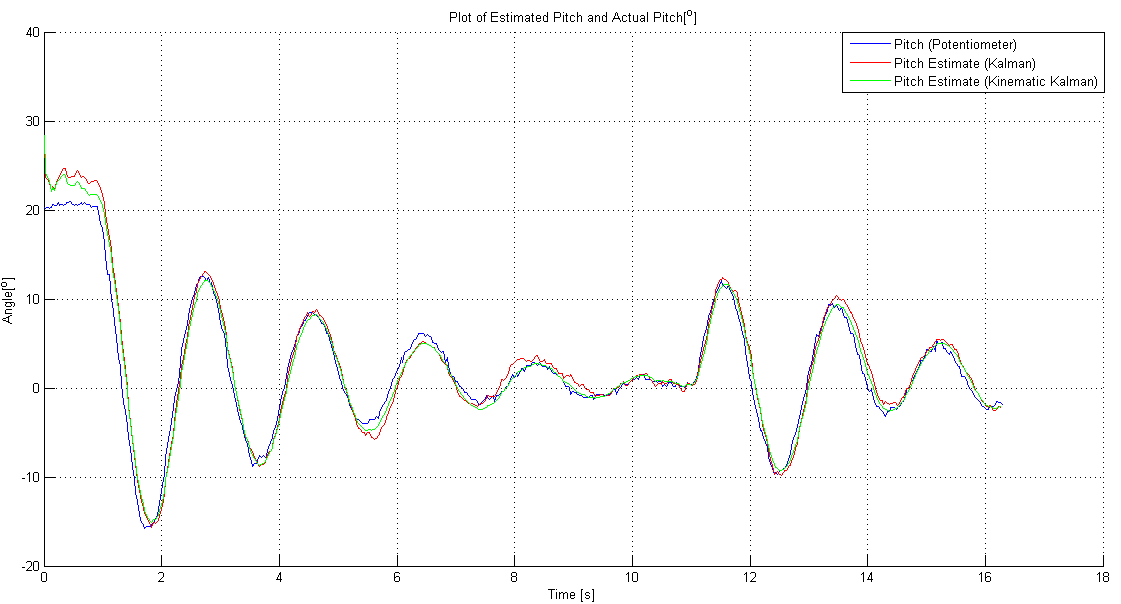
\includegraphics[width =0.7\paperwidth, height = 10cm]{\DocRoot/images/kalman_filter_comparsion}
							\caption{Plot of Kalman Filter Estimate, Kinematic Kalman Filter Estimate and Actual Angle of the device}
							\label{Fig: Kalman Filter Estimate and Kinematic Kalman Filter Estimate}
						\end{figure}




 \tocless\section{Introduction to the \gls{ekf} and associated code}
As the measurement function $h(x_k,\gls{noiseinoutput}_k)$ of the gyroscope is a non-linear function it was decided that it might be worth while looking at a more advanced kalman filter which is capable of dealing with non-linear systems, thus the \gls{ekf} was explore. Note as the group wanted to implement a \gls{gps} system on the quad-rotor the \gls{ekf} was the natural choice as it is the de-facto filter used in \gls{gps} systems \cite{An_Introduction_to_the_Kalman_Filter}. 


In something akin to a Taylor series, one most linearise the system around the current
estimate using the partial derivatives of the process and measurement functions to
compute estimates even in the face of non-linear relationships. The process is governed by the \textit{non-linear} stochastic difference equation:-
\begin{equation}
x_k = f(x_{k-1},u_k,\gls{noiseinsysystem}_{k-1})
\end{equation}
and the measurement model by the following stochastic difference equation:-
\begin{equation}
z_k = h(x_k,\gls{noiseinoutput}_k)
\end{equation}

where the random variables \gls{noiseinsysystem} and \gls{noiseinoutput} again represent the process and measurement
noise.



In practice of course one does not know the individual values of the noise \gls{noiseinsysystem} and \gls{noiseinoutput}  at
each time step. However, one can approximate the state and measurement  without
them as follows:-

\begin{equation}
x_k^* = f(\hat{x}_{k-1},u_k,0) \label{eq: ekf approximate the state }
\end{equation}
and the measurement model by the following stochastic difference equation:-
\begin{equation}
z_k = h(x_k^*,0)  \label{eq: ekf approximate the measurement}
\end{equation}

It is important to note that a fundamental flaw of the \gls{ekf} is that the distributions of the various random variables are no longer normal
after undergoing their respective non-linear transformations. The \gls{ekf} is simply an ad-hoc
state estimator that only approximates the optimality of Bayes’ rule by linearisation.


\eqref{eq: ekf approximate the state } is linearised around the control input $u_k$ and the previous estimate using \eqref{eq: jacobain of fx} and the measurement function \eqref{eq: ekf approximate the measurement} is linearised around the $x_k^*$  using  \eqref{eq: jacobain of hx}
\begin{equation}
A_k=\left.\left[\begin{array}{cccc}
\frac{\partial f_{1}}{\partial x_1} &\frac{\partial f_{1}}{\partial x_2} &\dots& \frac{\partial f_{1}}{\partial x_n}\\
\frac{\partial f_{2}}{\partial x_1} &\frac{\partial f_{2}}{\partial x_2} &\dots& \frac{\partial f_{2}}{\partial x_n}\\
\vdots& \vdots& \ddots &\vdots\\
\frac{\partial f_{n}}{\partial x_1} &\frac{\partial f_{n}}{\partial x_2} &\dots&\frac{\partial f_{n}}{\partial x_n} \\
\end{array}\right]\right|_{\hat{x}_k,u_k} \label{eq: jacobain of fx}
\end{equation}

\begin{equation}
C_k=\left.\left[\begin{array}{cccc}
\frac{\partial h_{1}}{\partial x_1} &\frac{\partial h_{1}}{\partial x_2} &\dots& \frac{\partial h_{1}}{\partial x_n}\\
\frac{\partial h_{2}}{\partial x_1} &\frac{\partial h_{2}}{\partial x_2} &\dots& \frac{\partial h_{2}}{\partial x_n}\\
\vdots& \vdots& \ddots &\vdots\\
\frac{\partial h_{n}}{\partial x_1} &\frac{\partial h_{n}}{\partial x_2} &\dots&\frac{\partial h_{n}}{\partial x_n} \\
\end{array}\right]\right|_{\hat{x}_k^*} \label{eq: jacobain of hx}
\end{equation}

Note the above Jacobian can be calculated at each stage on a micro-controller by using the Cauchy’s integral
formula which is defined as follows\cite{Jacobain_approx_paper}:-


\begin{equation}
f^{(n)}(z) = \frac{n!}{2\pi i}\oint_\gamma \frac{f(\kappa)}{(\kappa - z)^{n+1}}d\kappa \label{eq: Cauchy's intrgral formula}
\end{equation}

If one wants to implement \eqref{eq: Cauchy's intrgral formula} on a micro-controller one has to approximated it a closed form power series as follows:-

\begin{equation}
f^{(n)}(z) \approx \frac{n!}{mh} \sum_{j=0}^{m-1}\frac{f(z+h e^{i\frac{2 \pi j}{m}})}{e^{i\frac{2 \pi j n}{m}}}
\end{equation}

The derivation of a complex-step derivative (first partial derivative) approximation is done by an approximation of a non-linear function with a complex variable using the Taylor's series expansion.

\begin{equation}
f(x+ih) = f(x) + ihf^{'} (x) - h^2\frac{f^{''}(x)}{2!}- ih^3\frac{f^{'''}(x)}{3!}+h^4\frac{f^{4}(x)}{4!} + \dots
\end{equation}

Now taking only the imaginary parts of both sides gives
\begin{equation}
\mathrm{Im}[f(x+ih)] = hf^{'}(x) - h^3\frac{f^{'''}(x)}{3!}+\dots \label{eq: imaginary parts of  Cauchys integral approx}
\end{equation}
Dividing by $h$, rearranging and assuming terms higher than $h^2$ or higher can be ignored since the interval $h$ can be chosen up to the precision of the machine (smallest difference the machine can produce) and thus \eqref{eq: imaginary parts of  Cauchys integral approx} can be approximated as follows:-
\begin{equation}
f^{'}(x) = \mathrm{Im}[f(x+ih)]/h \label{eq: how to do differenation on a controller}
\end{equation}
As \eqref{eq: how to do differenation on a controller} is not a function of differences it is more accurate than standard finite difference and more inportantly one can now calculate a  partial derivative on a micro-controller using \eqref{eq: how to do differenation on a controller} 


	 \tocless\section{Chart Depicting how the \gls{ekf} Works}
	\begin{center}
		\begin{tikzpicture}[scale=0.65, transform shape]
		
		%
		% Styles for states, and state edges
		%
		\tikzstyle{state} = [{rectangle, rounded corners, draw=black, very thick, text width=20.0em, minimum height=4em, text centered}]
		\tikzstyle{stateEdgePortion} = [black,thick];
		\tikzstyle{stateEdge} = [stateEdgePortion,->];
		\tikzstyle{edgeLabel} = [pos=0.5, text centered, font={\sffamily\small}];
		
		
		%
		% Position States
		%
		\node[state, name=predict] {{{\LARGE}{\bf Model Update} (\enquote{Predict})}   \\ 
			{   (1) Predict State  \\  \vspace{-0.25cm}
				\hh $\hat{x}^{*}_{k} = f(\hat{x}_{k-1},u_k,0)$\\ 
				(2) Predict Error Covariance \\ \vspace{-0.25cm}
				\hh $\gls{covariancematrix}^* = A_k\gls{covariancematrix}_{-1}A_k^{\intercal} + \gls{couplingmatrix}_k\gls{noisecoplantmatrix}\gls{couplingmatrix}_k^{\intercal}$}};
				
				
				\node[state, name=correct, right of=predict, xshift=20em] {{\bf Measurement Update} (\enquote{Correct}) \\ 
					{   (1) Compute Kalman Gain\\  \vspace{-0.25cm}
						\hh $\gls{kalmangain}_{k} = \gls{covariancematrix}^*\gls{Cmatrix}_k^{\intercal}(\gls{Cmatrix}_k\gls{covariancematrix}^*\gls{Cmatrix}_k^{\intercal} + \gls{couplingmatrixoutput}_k\gls{noisecomatrix}_k\gls{couplingmatrixoutput}_k^{\intercal})^{-1}$\\ 
						(2) Update Estimate with Measurement $\gls{measurement}$ \\ \vspace{-0.25cm}
						\hh $\hat{x}_k = \hat{x}^{*}_k + \gls{kalmangain}_k(z_k - h(\hat{x}^{*}_{k},0))$\\
						(3) Update Error Covariance  \\ \vspace{-0.25cm}
						\hh $\gls{covariancematrix} = (I - \gls{kalmangain}_k\gls{Cmatrix}_k)\gls{covariancematrix}^{*}$
						
						}};
						
						
						%
						% Connect States via edges
						%
						\draw (predict.north) 
						edge[stateEdge, bend left=45] node[edgeLabel, xshift=-3em]{} 
						(correct.north); 
						
						\draw ($(predict.west) + (0,2.5em)$) 
						edge[stateEdgePortion] node[edgeLabel, yshift=+2.1cm]{} 
						($(predict.east) + (0,2.5em)$); 
						
						\draw (correct.south) 
						edge[stateEdge, bend left=45] node[edgeLabel, xshift=-3em]{} 
						(predict.south); 
						
						\draw ($(correct.west) + (0,4.0em)$) 
						edge[stateEdgePortion] node[edgeLabel, yshift=+2.1cm]{} 
						($(correct.east) + (0,4.0em)$); 
						
						
						
						% 
						% inital states to start the filter
						%
						\node[ name=inital, below of=predict, left of=predict, xshift = -3em ,yshift=-8em]{Initial Estimates for $\hat{x}_{k-1}$ and $\gls{covariancematrix}_{-1}$};
						
						\draw ($(inital.north) + (0,0)$) 
						edge[stateEdge] node[edgeLabel, yshift=+2.1cm]{} 
						($(predict.south) + (-5.4em,0)$); 
						\end{tikzpicture}
						\end{center}
